% questions.tex —— 2000 年·春季京皖卷·理科 · 题目内容片段（无答案）
% 由 tools/generate_projects.py 依来源总账自 2000/2000_数学真题_春季京皖理_试题.md 生成，勿手改（改源 MD 后重跑）


\gkpart{数学}

\begin{gktip}
\textbf{来源说明}：依据固定源 PDF 的原生文字层逐题转录，并对照 300 dpi 渲染与内容流核对（补集上划线、向量箭头、根号横、分数线为矢量短线，不在文字层）。源为 \textbf{XeTeX 重排件（非扫描）}，2 页 A3 横向三栏，页脚印刷页码 61、62；无答案页。题号 1–24 连续：选择 1–14、填空 15–18、解答 19–24。

\textbf{源内疑点}（照录不补正）：第 18 题 ③ 原页作「都有垂直」（「都」与「有」之间无停顿），疑为「都垂直」之误，照录不补正；第 23 题「年用电量为 a kW·h 本年度计划…」与「0.4 元/kW·h 经测算…」两处缺标点，原页如此，照录未补。

\textbf{图示}：第 14 题三次函数图象、第 20 题折叠三视图（3 幅）、第 22 题抛物线、第 24 题作图坐标系均由源内容流逐路径重绘，线宽/虚线按源值。
\end{gktip}

\gkpart{一、选择题}

\begin{question}
\gkti{1}复数 $z_1 = 3 + \mathrm{i}$，$z_2 = 1 - \mathrm{i}$，则 $z = z_1 \cdot z_2$ 在复平面内的对应点位于　（　）

\begin{gkopts}(4)
\task （A）第一象限
\task （B）第二象限
\task （C）第三象限
\task （D）第四象限
\end{gkopts}

\end{question}
\begin{question}
\gkti{2}设全集 $I = \{a, b, c, d, e\}$，集合 $M = \{a, c, d\}$，$N = \{b, d, e\}$，那么 $\overline{M} \cap \overline{N}$ 是　（　）

\begin{gkopts}(4)
\task （A）$\varnothing$
\task （B）$\{d\}$
\task （C）$\{a, c\}$
\task （D）$\{b, e\}$
\end{gkopts}

\end{question}
\begin{question}
\gkti{3}已知双曲线 $\frac{x^2}{b^2} - \frac{y^2}{a^2} = 1$ 的两条渐近线互相垂直，那么该双曲线的离心率是　（　）

\begin{gkopts}(4)
\task （A）$2$
\task （B）$\sqrt{3}$
\task （C）$\sqrt{2}$
\task （D）$\frac{3}{2}$
\end{gkopts}

\end{question}
\begin{question}
\gkti{4}曲线 $xy = 1$ 的参数方程是　（　）

（A）$\begin{cases} x = t^{\frac{1}{2}}, \\ y = t^{-\frac{1}{2}}. \end{cases}$　（B）$\begin{cases} x = \sin\alpha, \\ y = \csc\alpha. \end{cases}$

（C）$\begin{cases} x = \cos\alpha, \\ y = \sec\alpha. \end{cases}$　（D）$\begin{cases} x = \tan\alpha, \\ y = \cot\alpha. \end{cases}$

\end{question}
\begin{question}
\gkti{5}一个圆锥的底面直径和高都同一个球的直径相等，那么圆锥与球的体积之比是　（　）

\begin{gkopts}(4)
\task （A）$1:3$
\task （B）$2:3$
\task （C）$1:2$
\task （D）$2:9$
\end{gkopts}

\end{question}
\begin{question}
\gkti{6}直线 $\theta = a$ 和直线 $\rho\sin(\theta - a) = 1$ 的位置关系是　（　）

\begin{gkopts}(2)
\task （A）垂直
\task （B）平行
\task （C）相交但不垂直
\task （D）重合
\end{gkopts}

\end{question}
\begin{question}
\gkti{7}函数 $y = \lg |x|$　（　）

（A）是偶函数，在区间 $(-\infty, 0)$ 上单调递增

（B）是偶函数，在区间 $(-\infty, 0)$ 上单调递减

（C）是奇函数，在区间 $(0, +\infty)$ 上单调递增

（D）是奇函数，在区间 $(0, +\infty)$ 上单调递减

\end{question}
\begin{question}
\gkti{8}从单词“equation”选取 5 个不同的字母排成一排，含有“qu”（其中“qu”相连且顺序不变）的不同排列共有　（　）

\begin{gkopts}(4)
\task （A）120 个
\task （B）480 个
\task （C）720 个
\task （D）840 个
\end{gkopts}

\end{question}
\begin{question}
\gkti{9}椭圆短轴长是 2，长轴长是短轴的 2 倍，则椭圆中心到其准线距离是　（　）

\begin{gkopts}(2)
\task （A）$\frac{8}{5}\sqrt{5}$
\task （B）$\frac{4}{5}\sqrt{5}$
\task （C）$\frac{8}{3}\sqrt{3}$
\task （D）$\frac{4}{3}\sqrt{3}$
\end{gkopts}

\end{question}
\begin{question}
\gkti{10}函数 $y = \dfrac{1}{2 + \sin x + \cos x}$ 的最大值是　（　）

\begin{gkopts}(2)
\task （A）$\dfrac{\sqrt{2}}{2} - 1$
\task （B）$\dfrac{\sqrt{2}}{2} + 1$
\task （C）$1 - \dfrac{\sqrt{2}}{2}$
\task （D）$-1 - \dfrac{\sqrt{2}}{2}$
\end{gkopts}

\end{question}
\begin{question}
\gkti{11}设复数 $z_1 = 2\sin\theta + \mathrm{i}\cos\theta$（$\frac{\pi}{4} < \theta < \frac{\pi}{2}$）在复平面上对应向量 $\overrightarrow{OZ_1}$，将 $\overrightarrow{OZ_1}$ 按顺时针方向旋转 $\frac{3}{4}\pi$ 后得到向量 $\overrightarrow{OZ_2}$，$\overrightarrow{OZ_2}$ 对应的复数为 $z_2 = r(\cos\varphi + \mathrm{i}\sin\varphi)$，则 $\tan\varphi =$　（　）

\begin{gkopts}(2)
\task （A）$\frac{2\tan\theta + 1}{2\tan\theta - 1}$
\task （B）$\frac{2\tan\theta - 1}{2\tan\theta + 1}$
\task （C）$\frac{1}{2\tan\theta + 1}$
\task （D）$\frac{1}{2\tan\theta - 1}$
\end{gkopts}

\end{question}
\begin{question}
\gkti{12}设 $\alpha$，$\beta$ 是一个钝角三角形的两个锐角，下列四个不等式中不正确的是　（　）

（A）$\tan\alpha\tan\beta < 1$　（B）$\sin\alpha + \sin\beta < \sqrt{2}$

（C）$\cos\alpha + \cos\beta > 1$　（D）$\frac{1}{2}\tan(\alpha+\beta) < \tan\frac{\alpha+\beta}{2}$

\end{question}
\begin{question}
\gkti{13}已知等差数列 $\{a_n\}$ 满足 $a_1 + a_2 + a_3 + \cdots + a_{101} = 0$，则有　（　）

\begin{gkopts}(2)
\task （A）$a_1 + a_{101} > 0$
\task （B）$a_2 + a_{100} < 0$
\task （C）$a_3 + a_{99} = 0$
\task （D）$a_{51} = 51$
\end{gkopts}

\Needspace{0.4\textheight}
\end{question}
\begin{question}
\gkti{14}已知函数 $f(x) = ax^3 + bx^2 + cx + d$ 的图象如图，则　（　）
\nopagebreak[4]
\begin{center}% f2000_spring_jingwan_science_q14_graph.tex — 2000 年·春季京皖卷·理科 第 14 题（f(x)=ax³+bx²+cx+d 的图象）
%
% 【来源】`.work/phase4-b20/source/2000春季京皖理.pdf`
%   （SHA-256 37f07244497aa0a21be12d8a31eac78b61490f835f088719a5990463585a35ce），
%   第 1 页（印刷页 61）；qpdf --qdf 解包后对内容流逐路径解析。
% 【坐标口径】源 PDF 用户空间（原点左下、y 向上）。本图本地坐标
%   (x, y) = (x_page − 608.528, y_page − 518.047)，1 单位 = 1 TeX pt；
%   O 取两轴交点；x 轴 y_page ≡ 518.047，y 轴 x_page ≡ 608.528。
% 【元素计数】5 条路径（x 轴／x 箭头／y 轴／y 箭头／曲线）＋ 5 个标签。
% 【标签】位置取 pdftotext -bbox 文本中心换算（源中心逐条记在 \node 行末）；
%   本图有 3 处微调（源位与微调量见各 \node 行末）：「O」左移 2.2 pt 避曲线，
%   「1」「2」同步下移 2.56 pt（保持两刻度同基线；「2」原净距仅 1.0 pt）。
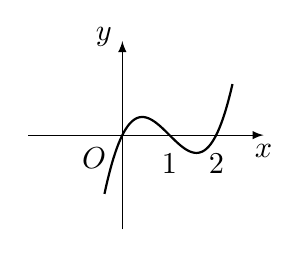
\begin{tikzpicture}[x=1pt, y=1pt,
    every node/.style={inner sep=0pt, font=\fontsize{10.5pt}{12.6pt}\selectfont}]
  \draw[line width=0.399pt] (-34.017,0) -- (47.438,0);
  \fill[line width=0.399pt] (51.025,0) .. controls (49.962,0.199) and (48.235,0.797) .. (47.04,1.494) -- (47.04,-1.494) .. controls (48.235,-0.797) and (49.962,-0.199) .. (51.025,0);
  \draw[line width=0.399pt] (0,-34.017) -- (0,30.43);
  \fill[line width=1.000pt] (0,34.016) .. controls (-0.199,32.954) and (-0.797,31.227) .. (-1.494,30.031) -- (1.494,30.031) .. controls (0.797,31.227) and (0.199,32.954) .. (0,34.016);
  % 曲线（本图第 5 条路径）：7177 个采样点 / 299 段三次贝塞尔。最小二乘拟合
  %   y = 0.003457x^3 - 0.176384x^2 + 1.999983x（rms 0.0002 pt，最大偏差 0.0025 pt），按该式绘制。
  \draw[line width=0.797pt, domain=-6.4632:39.7852, samples=240]
    plot (\x, {0.003457*\x*\x*\x - 0.176384*\x*\x + 1.999983*\x});

  \node[anchor=center] at (-6.648,35.403) {$y$};  % 源中心 (601.88,553.45)
  \node[anchor=center] at (-10.198,-8.247) {$O$};  % 源中心 (600.53,509.80)；左移 2.2 pt 避曲线（原净距 1.0 pt）
  \node[anchor=center] at (17.012,-10.397) {$1$};  % 源中心 (625.54,510.21)；与 2 同步下移 2.56 pt 保持同基线
  \node[anchor=center] at (34.012,-10.397) {$2$};  % 源中心 (642.54,510.21)；下移 2.56 pt 避曲线（原净距 1.0 pt）
  \node[anchor=center] at (51.022,-5.597) {$x$};  % 源中心 (659.55,512.45)
\end{tikzpicture}
%
% 【自验】
%   1) 探针编译：/tmp 最小文档（ctexart + common/preamble + xelatex）\input 本文件，0 error、0 warning。
%   2) 600 dpi 双渲染差分（有标签 / 标签 opacity=0）量测标签墨迹到路径墨迹最近距离：
%      各标签净距：「2」2.80、「x」2.85、「O」3.06、「1」4.35、「y」5.24 —— 最小 2.80 pt。
%   3) 线形：两轴 0.399 pt，曲线 0.797 pt，实线，与源 w 值一致；箭头为源贝塞尔填充路径。
%   4) 曲线拟合残差 rms 0.0002 pt、最大 0.0025 pt；根 x=0、17.00、34.02 与源标注 1、2 对位。
\end{center}
\nopagebreak[4]
\begin{gkopts}(2)
\task （A）$b \in (-\infty, 0)$
\task （B）$b \in (0, 1)$
\task （C）$b \in (1, 2)$
\task （D）$b \in (2, +\infty)$
\end{gkopts}

\end{question}
\gkpart{二、填空题}

\begin{question}
\gkti{15}函数 $y = \cos\left(\frac{2\pi}{3}x + \frac{\pi}{4}\right)$ 的最小正周期是\gkblank{}．

\end{question}
\begin{question}
\gkti{16}已知一体积为 72 的正四面体，连结两个面的重心 $E$、$F$，则线段 $EF$ 的长是\gkblank{}．

\end{question}
\begin{question}
\gkti{17}$\left(\sqrt{x} - \frac{1}{\sqrt[3]{x}}\right)^{10}$ 展开式中的常数项是\gkblank{}．

\end{question}
\begin{question}
\gkti{18}在空间，下列命题正确的是\gkblank{}．（注：把你认为正确的命题的序号都填上）

① 如果两直线 $a$、$b$ 分别与直线 $l$ 平行，那么 $a \parallel b$；

② 如果直线 $a$ 与平面 $\beta$ 内的一条直线 $b$ 平行，那么 $a \parallel \beta$；

③ 如果直线 $a$ 与平面 $\beta$ 内的两条直线 $b$、$c$ 都有垂直，那么 $a \perp \beta$；

④ 如果平面 $\beta$ 内的一条直线 $a$ 垂直平面 $\gamma$，那么 $\beta \perp \gamma$．

\end{question}
\gkpart{三、解答题}

\begin{question}
\gkti{19}在 $\triangle ABC$ 中，角 $A$、$B$、$C$ 对边分别为 $a$、$b$、$c$，证明：$\dfrac{a^2 - b^2}{c^2} = \dfrac{\sin(A - B)}{\sin C}$．

\Needspace{0.4\textheight}
\end{question}
\begin{question}
\gkti{20}在直角梯形 $ABCD$ 中，$\angle D = \angle BAD = 90^\circ$，$AD = DC = \frac{1}{2}AB = a$（如图一）．将 $\triangle ADC$ 沿 $AC$ 折起，使 $D$ 到 $D'$．记面 $ACD'$ 为 $\alpha$，面 $ABC$ 为 $\beta$，面 $BCD'$ 为 $\gamma$．

（1） 若二面角 $\alpha-AC-\beta$ 为直二面角（如图二），求二面角 $\beta-BC-\gamma$ 的大小；

（2） 若二面角 $\alpha-AC-\beta$ 为 $60^\circ$（如图三），求三棱锥 $D'-ABC$ 的体积．
\nopagebreak[4]
\begin{center}% f2000_spring_jingwan_science_q20_fig1.tex — 2000 年·春季京皖卷·理科 第 20 题 图一（直角梯形 ABCD，虚线 AC）
%
% 【来源】`.work/phase4-b20/source/2000春季京皖理.pdf`
%   （SHA-256 37f07244497aa0a21be12d8a31eac78b61490f835f088719a5990463585a35ce），
%   第 1 页（印刷页 61）；qpdf --qdf 解包后对内容流逐路径解析。
% 【坐标口径】源 PDF 用户空间（原点左下、y 向上）。本图本地坐标
%   (x, y) = (x_page − 832.206, y_page − 629.419)，1 单位 = 1 TeX pt；
%   A 取梯形左下顶点；AB 水平（y_page ≡ 629.419），AD 铅直（x_page ≡ 832.206）。
% 【元素计数】5 条路径（AB／BC／CD／DA／AC 虚线）＋ 4 个标签。
% 【标签】位置取 pdftotext -bbox 文本中心换算（源中心逐条记在 \node 行末）；
%   本图有 1 处微调：「C」上移 1.5 pt，避开梯形上底 CD（原净距 1.8 pt）；
%   其余标签按源中心放置。
\begin{tikzpicture}[x=1pt, y=1pt,
    every node/.style={inner sep=0pt, font=\fontsize{10.5pt}{12.6pt}\selectfont}]
  \draw[line width=0.399pt] (0,0) -- (68.037,0);
  \draw[line width=0.399pt] (68.037,0) -- (34.019,34.019);
  \draw[line width=0.399pt] (34.019,34.019) -- (0,34.019);
  \draw[line width=0.399pt] (0,34.019) -- (0,0);
  \draw[line width=0.399pt, dash pattern=on 2.99pt off 2.99pt] (0,0) -- (34.019,34.019);

  \node[anchor=center] at (-4.936,-5.889) {$A$};  % 源中心 (827.27,623.53)
  \node[anchor=center] at (72.704,-5.889) {$B$};  % 源中心 (904.91,623.53)
  \node[anchor=center] at (38.574,39.491) {$C$};  % 源中心 (870.78,667.41)；上移 1.5 pt 避 CD 边（原净距 1.8 pt）
  \node[anchor=center] at (-5.076,37.991) {$D$};  % 源中心 (827.13,667.41)
  % 图注（源页图下居中）
  \node at (34.019,-12.000) {图一};
\end{tikzpicture}
%
% 【自验】
%   1) 探针编译：0 error、0 warning。
%   2) 600 dpi 双渲染差分量测标签净距：C 2.90、D 3.05、B 3.49、A 3.50 —— 最小 2.90 pt。
%   3) 线形：实线 4 条 0.399 pt，虚线 AC 用源实测节距 dash pattern=on 2.99pt off 2.99pt；
%      600 dpi 下沿 AC 数得 9 节（8 整节 + 末端 0.5 pt 残节），与源 PDF 同法计数一致。
\end{center}
\nopagebreak[4]
\nopagebreak[4]
\begin{center}% f2000_spring_jingwan_science_q20_fig2.tex — 2000 年·春季京皖卷·理科 第 20 题 图二（折叠后三棱锥 D′-ABC，直二面角）
%
% 【来源】`.work/phase4-b20/source/2000春季京皖理.pdf`
%   （SHA-256 37f07244497aa0a21be12d8a31eac78b61490f835f088719a5990463585a35ce），
%   第 1 页（印刷页 61）；qpdf --qdf 解包后对内容流逐路径解析。
% 【坐标口径】源 PDF 用户空间（原点左下、y 向上）。本图本地坐标
%   (x, y) = (x_page − 949.762, y_page − 629.419)，1 单位 = 1 TeX pt；
%   A 取底面左端点；AB 水平（y_page ≡ 629.419）。
% 【元素计数】6 条路径（AB／BD′／D′A 实线；AC／CB／CD′ 虚线）＋ 4 个标签。
% 【标签】位置取 pdftotext -bbox 文本中心换算（源中心逐条记在 \node 行末）；
%   本图有 1 处微调：「C」下移 3.0 pt，避开 AC 虚线（原净距 2.0 pt）；
%   其余标签按源中心放置。
\begin{tikzpicture}[x=1pt, y=1pt,
    every node/.style={inner sep=0pt, font=\fontsize{10.5pt}{12.6pt}\selectfont}]
  \draw[line width=0.399pt] (0,0) -- (68.037,0);
  \draw[line width=0.399pt] (68.037,0) -- (17.009,34.019);
  \draw[line width=0.399pt] (17.009,34.019) -- (0,0);
  \draw[line width=0.399pt, dash pattern=on 2.99pt off 2.99pt] (0,0) -- (20.411,20.411);
  \draw[line width=0.399pt, dash pattern=on 2.99pt off 2.99pt] (68.037,0) -- (20.411,20.411);
  \draw[line width=0.399pt, dash pattern=on 2.99pt off 2.99pt] (20.411,20.411) -- (17.009,34.019);

  \node[anchor=center] at (-4.932,-5.889) {$A$};  % 源中心 (944.83,623.53)
  \node[anchor=center] at (72.708,-5.889) {$B$};  % 源中心 (1022.47,623.53)
  \node[anchor=center] at (20.038,9.471) {$C$};  % 源中心 (969.80,641.89)；下移 3.0 pt 避 AC 虚线（原净距 2.0 pt）
  \node[anchor=center] at (16.758,41.351) {$D'$};  % 源中心 (966.52,670.77)；取 D 与标注撇号合框中心
  % 图注（源页图下居中）
  \node at (34.019,-12.000) {图二};
\end{tikzpicture}
%
% 【自验】
%   1) 探针编译：0 error、0 warning。
%   2) 600 dpi 双渲染差分量测标签净距：B 3.48、A 3.56、D′ 3.64、C 4.07 —— 最小 3.48 pt。
%   3) 线形：AB／AD′／BD′ 实线 0.399 pt；AC／CB／CD′ 虚线节距 on 2.99pt off 2.99pt（源 d=[2.99 2.99]）。
\end{center}
\nopagebreak[4]
\nopagebreak[4]
\begin{center}% f2000_spring_jingwan_science_q20_fig3.tex — 2000 年·春季京皖卷·理科 第 20 题 图三（折叠后三棱锥 D′-ABC，二面角 60°）
%
% 【来源】`.work/phase4-b20/source/2000春季京皖理.pdf`
%   （SHA-256 37f07244497aa0a21be12d8a31eac78b61490f835f088719a5990463585a35ce），
%   第 1 页（印刷页 61）；qpdf --qdf 解包后对内容流逐路径解析。
% 【坐标口径】源 PDF 用户空间（原点左下、y 向上）。本图本地坐标
%   (x, y) = (x_page − 1067.319, y_page − 629.419)，1 单位 = 1 TeX pt；
%   A 取底面左端点；AB 水平（y_page ≡ 629.419）。
% 【元素计数】6 条路径（AB／BD′／D′A 实线；AC／CB／CD′ 虚线）＋ 4 个标签。
% 【标签】位置取 pdftotext -bbox 文本中心换算（源中心逐条记在 \node 行末）；
%   本图有 1 处微调：「C」下移 3.0 pt，避开 AC 虚线（原净距 2.0 pt）；
%   其余标签按源中心放置。
\begin{tikzpicture}[x=1pt, y=1pt,
    every node/.style={inner sep=0pt, font=\fontsize{10.5pt}{12.6pt}\selectfont}]
  \draw[line width=0.399pt] (0,0) -- (68.037,0);
  \draw[line width=0.399pt] (68.037,0) -- (25.514,34.019);
  \draw[line width=0.399pt] (25.514,34.019) -- (0,0);
  \draw[line width=0.399pt, dash pattern=on 2.99pt off 2.99pt] (0,0) -- (20.411,20.411);
  \draw[line width=0.399pt, dash pattern=on 2.99pt off 2.99pt] (68.037,0) -- (20.411,20.411);
  \draw[line width=0.399pt, dash pattern=on 2.99pt off 2.99pt] (20.411,20.411) -- (25.514,34.019);

  \node[anchor=center] at (-4.929,-5.889) {$A$};  % 源中心 (1062.39,623.53)
  \node[anchor=center] at (72.701,-5.889) {$B$};  % 源中心 (1140.02,623.53)
  \node[anchor=center] at (20.031,9.471) {$C$};  % 源中心 (1087.35,641.89)；下移 3.0 pt 避 AC 虚线（原净距 2.0 pt）
  \node[anchor=center] at (25.271,41.351) {$D'$};  % 源中心 (1092.59,670.77)；取 D 与标注撇号合框中心
  % 图注（源页图下居中）
  \node at (34.019,-12.000) {图三};
\end{tikzpicture}
%
% 【自验】
%   1) 探针编译：0 error、0 warning。
%   2) 600 dpi 双渲染差分量测标签净距：B 3.48、A 3.56、D′ 3.68、C 4.07 —— 最小 3.48 pt。
%   3) 线形：AB／AD′／BD′ 实线 0.399 pt；AC／CB／CD′ 虚线节距 on 2.99pt off 2.99pt（源 d=[2.99 2.99]）。
\end{center}
\nopagebreak[4]
\end{question}
\begin{question}
\gkti{21}设函数 $f(x) = |\lg x|$，若 $0 < a < b$，且 $f(a) > f(b)$，证明：$ab < 1$．

\Needspace{0.4\textheight}
\end{question}
\begin{question}
\gkti{22}如图，设点 $A$ 和 $B$ 为抛物线 $y^2 = 4px$（$p > 0$）上原点以外的两个动点，已知 $OA \perp OB$，$OM \perp AB$．求点 $M$ 的轨迹方程，并说明它表示什么曲线．
\nopagebreak[4]
\begin{center}% f2000_spring_jingwan_science_q22_parabola.tex — 2000 年·春季京皖卷·理科 第 22 题（抛物线 y²=4px 与动点 A、B、M）
%
% 【来源】`.work/phase4-b20/source/2000春季京皖理.pdf`
%   （SHA-256 37f07244497aa0a21be12d8a31eac78b61490f835f088719a5990463585a35ce），
%   第 2 页（印刷页 62）；qpdf --qdf 解包后对内容流逐路径解析。
% 【坐标口径】源 PDF 用户空间（原点左下、y 向上）。本图本地坐标
%   (x, y) = (x_page − 329.307, y_page − 687.581)，1 单位 = 1 TeX pt；
%   O 取两轴交点；x 轴 y_page ≡ 687.581，y 轴 x_page ≡ 329.307。
% 【元素计数】10 条绘制路径（x 轴／x 箭头／y 轴／y 箭头／AB／OA／OB／OM／抛物线上支／下支）＋ 6 个标签。
%   源内容流为 11 条：其中路径 6（直线 O→A）与路径 10（贝塞尔 O→A）几何重合，已合并。
% 【标签】位置取 pdftotext -bbox 文本中心换算（源中心逐条记在 \node 行末）；
%   本图各标签按源中心放置，无微调。
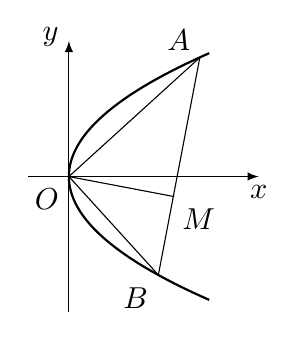
\begin{tikzpicture}[x=1pt, y=1pt,
    every node/.style={inner sep=0pt, font=\fontsize{10.5pt}{12.6pt}\selectfont}]
  \draw[line width=0.399pt] (-14.695,0) -- (64.989,0);
  \fill[line width=0.399pt] (68.576,0) .. controls (67.513,0.199) and (65.786,0.797) .. (64.591,1.494) -- (64.591,-1.494) .. controls (65.786,-0.797) and (67.513,-0.199) .. (68.576,0);
  \draw[line width=0.399pt] (0,-48.983) -- (0,45.396);
  \fill[line width=0.399pt] (0,48.983) .. controls (-0.199,47.92) and (-0.797,46.193) .. (-1.494,44.998) -- (1.494,44.998) .. controls (0.797,46.193) and (0.199,47.92) .. (0,48.983);
  % 三条割线。源内容流中 OB（路径 8）、OM（路径 9）以密集三次贝塞尔绘制，
  % 与直线最大偏差 0.0002 pt，此处按直线写出；O→A 另有路径 6（直线）与路径 10（贝塞尔）
  % 几何重合（偏差 < 0.01 pt），合并为一条。
  \draw[line width=0.399pt] (32.329,-35.562) -- (47.317,43.007);   % AB
  \draw[line width=0.399pt] (0,0) -- (47.317,43.007);              % OA
  \draw[line width=0.399pt] (0,0) -- (32.329,-35.562);             % OB
  \draw[line width=0.399pt] (0,0) -- (38.108,-7.269);              % OM
  % 抛物线 y^2 = 4px 的上、下两支（源路径 7 / 11，各 24 段三次贝塞尔）。
  % 拟合 x = 0.0255212 y^2（rms 0.0025 pt），即 4p = 39.177 pt。
  \draw[line width=0.797pt, domain=0:44.5724, samples=120, variable=\y]
    plot ({0.0255212*\y*\y}, \y);
  \draw[line width=0.797pt, domain=-44.5724:0, samples=120, variable=\y]
    plot ({0.0255212*\y*\y}, \y);

  \node[anchor=center] at (-6.647,50.369) {$y$};  % 源中心 (322.66,737.95)
  \node[anchor=center] at (39.683,49.329) {$A$};  % 源中心 (368.99,736.91)
  \node[anchor=center] at (68.573,-5.591) {$x$};  % 源中心 (397.88,681.99)
  \node[anchor=center] at (-7.997,-8.251) {$O$};  % 源中心 (321.31,679.33)
  \node[anchor=center] at (46.903,-15.521) {$M$};  % 源中心 (376.21,672.06)
  \node[anchor=center] at (24.123,-43.811) {$B$};  % 源中心 (353.43,643.77)
\end{tikzpicture}
%
% 【自验】
%   1) 探针编译：0 error、0 warning。
%   2) 600 dpi 双渲染差分量测标签净距：x 2.81、A 3.88、O 4.32、y 5.20、M 5.86、B 6.44 —— 最小 2.81 pt。
%   3) 线形：两轴与三条割线 0.399 pt；抛物线两支 0.797 pt，与源 w、d 值一致（全为实线）。
%   4) 抛物线拟合残差 rms 0.0025 pt；A、B 落在抛物线上（偏差 0.1 pt 内），OA⊥OB 斜率积 −1.000。
\end{center}
\nopagebreak[4]
\end{question}
\begin{question}
\gkti{23}某地区上年度电价为 $0.8$ 元/kW$\cdot$h，年用电量为 $a$ kW$\cdot$h　本年度计划将电价降到 $0.55$ 元/kW$\cdot$h 至 $0.75$ 元/kW$\cdot$h 之间，而用户期望电价为 $0.4$ 元/kW$\cdot$h　经测算，下调电价后新增的用电量与实际电价和用户期望电价的差成反比（比例系数为 $k$）．该地区电力的成本为 $0.3$ 元/kW$\cdot$h．

（1） 写出本年度电价下调后，电力部门的收益 $y$ 与实际电价 $x$ 的函数关系式；

（2） 设 $k = 0.2a$，当电价最低定为多少时仍可保证电力部门的收益比上年至少增长 $20\%$？

注：收益 = 实际用电量 ×（实际电价 $-$ 成本价）

\Needspace{0.4\textheight}
\end{question}
\begin{question}
\gkti{24}已知函数

\nopagebreak[4]
\[f(x) = \begin{cases} f_1(x), & x \in \left[0, \dfrac{1}{2}\right), \\[4pt] f_2(x), & x \in \left[\dfrac{1}{2}, 1\right], \end{cases} \qquad \text{\text{其中} } f_1(x) = -2\left(x - \dfrac{1}{2}\right)^2 + 1,\]

\nopagebreak[4]
\[f_2(x) = -2x + 2.\]

（1） 在下面坐标系上画出 $y = f(x)$ 的图象；
\nopagebreak[4]
\begin{center}% f2000_spring_jingwan_science_q24_grid.tex — 2000 年·春季京皖卷·理科 第 24 题（空白平面直角坐标系，供作图）
%
% 【来源】`.work/phase4-b20/source/2000春季京皖理.pdf`
%   （SHA-256 37f07244497aa0a21be12d8a31eac78b61490f835f088719a5990463585a35ce），
%   第 2 页（印刷页 62）；qpdf --qdf 解包后对内容流逐路径解析。
% 【坐标口径】源 PDF 用户空间（原点左下、y 向上）。本图本地坐标
%   (x, y) = (x_page − 1062.162, y_page − 536.238)，1 单位 = 1 TeX pt；
%   O 取两轴交点；两轴等长（−15.874…75.784 pt），刻度 0.5 间隔 31.748 pt、1 间隔 63.497 pt。
% 【元素计数】8 条路径（x 轴／x 箭头／y 轴／y 箭头／4 条刻度线）＋ 7 个标签。
% 【标签】位置取 pdftotext -bbox 文本中心换算（源中心逐条记在 \node 行末）；
%   本图各标签按源中心放置，无微调。
\begin{tikzpicture}[x=1pt, y=1pt,
    every node/.style={inner sep=0pt, font=\fontsize{10.5pt}{12.6pt}\selectfont}]
  \draw[line width=0.399pt] (-15.874,0) -- (75.784,0);
  \fill[line width=0.399pt] (79.371,0) .. controls (78.308,0.199) and (76.581,0.797) .. (75.386,1.494) -- (75.386,-1.494) .. controls (76.581,-0.797) and (78.308,-0.199) .. (79.371,0);
  \draw[line width=0.399pt] (0,-15.874) -- (0,75.784);
  \fill[line width=0.399pt] (0,79.371) .. controls (-0.199,78.308) and (-0.797,76.581) .. (-1.494,75.386) -- (1.494,75.386) .. controls (0.797,76.581) and (0.199,78.308) .. (0,79.371);
  \draw[line width=0.399pt] (31.748,0) -- (31.748,3.175);
  \draw[line width=0.399pt] (0,31.748) -- (3.175,31.748);
  \draw[line width=0.399pt] (63.497,0) -- (63.497,3.175);
  \draw[line width=0.399pt] (0,63.497) -- (3.175,63.497);

  \node[anchor=center] at (-6.652,80.752) {$y$};  % 源中心 (1055.51,616.99)
  \node[anchor=center] at (-6.322,62.742) {$1$};  % 源中心 (1055.84,598.98)
  \node[anchor=center] at (-10.412,30.992) {$0.5$};  % 源中心 (1051.75,567.23)
  \node[anchor=center] at (-7.992,-8.248) {$O$};  % 源中心 (1054.17,527.99)
  \node[anchor=center] at (31.748,-7.838) {$0.5$};  % 源中心 (1093.91,528.40)
  \node[anchor=center] at (63.498,-7.838) {$1$};  % 源中心 (1125.66,528.40)
  \node[anchor=center] at (79.368,-5.598) {$x$};  % 源中心 (1141.53,530.64)
\end{tikzpicture}
%
% 【自验】
%   1) 探针编译：0 error、0 warning。
%   2) 600 dpi 双渲染差分量测标签净距：x 2.79，x 轴「0.5」「1」各 4.08，O 4.32，
%      y 轴「0.5」4.20、「1」4.44、「y」5.26 —— 最小 2.79 pt。
%   3) 线形：两轴与 4 条刻度线均 0.399 pt 实线；刻度长 3.175 pt，与源一致。
%   4) 刻度间距：x 轴 31.748/63.497 pt，y 轴 31.748/63.497 pt，两轴等长 91.658 pt。
\end{center}
\nopagebreak[4]
（2） 设 $y = f_2(x)$（$x \in \left[\dfrac{1}{2}, 1\right]$）的反函数为 $y = g(x)$，$a_1 = 1$，$a_2 = g(a_1)$，$\cdots$，$a_n = g(a_{n-1})$，求数列 $\{a_n\}$ 的通项公式，并求 $\lim\limits_{n \to \infty} a_n$；

（3） 若 $x_0 \in \left[0, \dfrac{1}{2}\right)$，$x_1 = f(x_0)$，$f(x_1) = x_0$，求 $x_0$．

\par\medskip

\end{question}